\section{Experiments}

During development, the Discovery Service and Specification Retriever software were tested separately by mocking other elements in the Cloudify cluster. This section describes the experiments and their set-ups for 

\subsubsection{Hardware set-up}
To verify that the Discovery Service and the Specification retriever function correctly in real environment and on real machines, I set up a test-bed depicted in figure ~\ref{fig:network-venn}.

 \begin{figure}[ht!]
\centering
  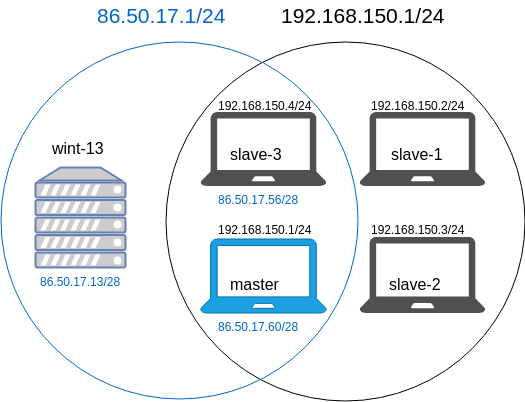
\includegraphics[width=12cm,height=12cm, keepaspectratio]{Network-venn.png}%
  \caption{The testbed hosts are located in a private network but master and slave-3 can also access internet via bastion host wint-13}
  \label{fig:network-venn}
\end{figure}

The test-bed consist of a Lenovo Thinkpad T420S 4173L7G laptop computer with  4-core Intel i5-2540M CPU and 8 GB of RAM acting as a master node in the Cloudify cluster. The three slave-machines are Lenovo Thinkpad Edge E145's with 2-core AMD E1-2500 APU CPUs and 4 GB of RAM. The master host has Centos 7 installed as the operating system to accommodate Cloudify's installation requirements. The three slave machines are running Ubuntu 16.04 as the OS of the slaves can be anything as long as they are Linux-based and the hosts themselves can be accessed via SSH.

As seen on figure ~\ref{fig:network-venn}, the test-bed set up has two different networks. The Master can be accessed remotely via a bastion host \textit{wint-13}. Wint-13 itself is not a part of the test-bed set up, but it is used to access the testbed remotely and allow internet access for the master host.

Master host has two network interfaces configure for each network it's a part of: The subnet 83.50.17.1 for outside access and 192.168.150.1 which is the subnet dedicated for the Cloudify cluster. Master also serves as a default gateway for all of the slaves. Figure ~\ref{fig:network-venn} shows how slave machines are part of the cluster subnet with static IP addresses. In addition slave-3 is also connected to the 83.50.17.1 subnet. This is to provide a way to drop the host off the cluster network but still be able to access it remotely via external network.

\subsubsection{Software environment set-up}